\documentclass[12pt]{article}
% This first part of the file is called the PREAMBLE. It includes
% customizations and command definitions. The preamble is everything
% between \documentclass and \begin{document}.

\usepackage[margin=1in]{geometry}  % set the margins to 1in on all sides
\usepackage{graphicx}              % to include figures
\usepackage{amsmath}               % great math stuff
\usepackage{amsfonts}              % for blackboard bold, etc
\usepackage{amsthm}                % better theorem environments

\usepackage{rotating} % for sideway table
\usepackage{xcolor}
\usepackage{hyperref}
\hypersetup{
    colorlinks,
    linkcolor={red!50!black},
    citecolor={blue!50!black},
    urlcolor={blue!80!black}
}
\usepackage{cleveref} % Reference
\usepackage{enumitem} % nosep

\usepackage{array,tabularx}

\newenvironment{conditions*}
  {\par\vspace{\abovedisplayskip}\noindent
   \tabularx{\columnwidth}{>{$}l<{$} @{${}={}$} >{\raggedright\arraybackslash}X}}
  {\endtabularx\par\vspace{\belowdisplayskip}}
  
\usepackage{float}
\restylefloat{table}

% various theorems, numbered by section

\newtheorem{thm}{Theorem}[section]
\newtheorem{lem}[thm]{Lemma}
\newtheorem{prop}[thm]{Proposition}
\newtheorem{cor}[thm]{Corollary}
\newtheorem{conj}[thm]{Conjecture}

\DeclareMathOperator{\id}{id}

\newcommand{\bd}[1]{\mathbf{#1}}  % for bolding symbols
\newcommand{\RR}{\mathbb{R}}      % for Real numbers
\newcommand{\ZZ}{\mathbb{Z}}      % for Integers
\newcommand{\col}[1]{\left[\begin{matrix} #1 \end{matrix} \right]}
\newcommand{\comb}[2]{\binom{#1^2 + #2^2}{#1+#2}}

% bibliography
\usepackage{natbib}
\bibpunct{(}{)}{;}{a}{}{,} % no comma between author and year

\title{Prospectus: The political determinants of FDI technological spillover and corruption}
\author{Anh Le}


\begin{document}
\maketitle

\section{Empirical Puzzle}
In recent decades, foreign direct investment (FDI) global flow has steadily increased, rising to over \$1.5 trillion dollars in 2014. For developing countries, FDI flow is also remarkably robust to global downturn, leading to enthusiastic endorsement by major international organizations as a key factor to economic development (\Cref{fig:globalfdi}).\footnote{http://www.imf.org/external/pubs/ft/fandd/1999/03/mallampa.htm, http://www.weforum.org/reports/foreign-direct-investment-key-driver-trade-growth-and-prosperity-case-multilateral-agreement} This assumption is also shared widely within political science, where much of the literature starts with the assumption that countries want to seek FDI for its many benefits. The question that these works focus on is \textit{how} countries can attract FDI, not \textit{whether} they want to do so \citep{Jensen2003, Li2003, Li2006, Ahlquist2006}.\footnote{Two recent exceptions are \citet{Pinto2013, Pandya2013}, which are the first to investigate the demand for FDI.} 

\begin{figure}[!ht]
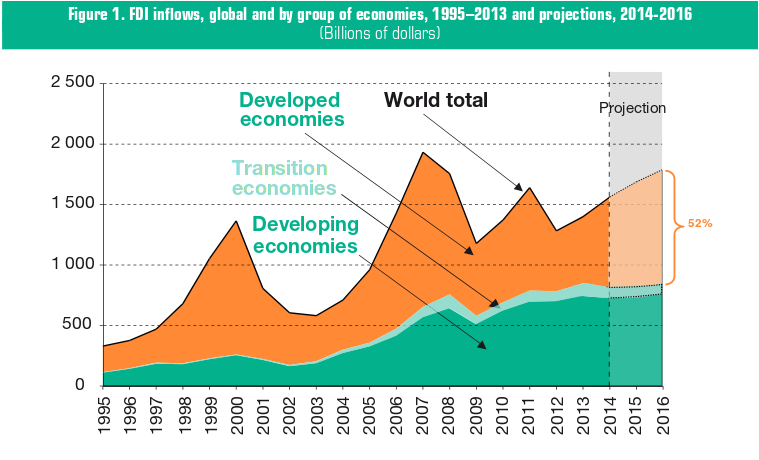
\includegraphics[width=\textwidth, height=\textheight,keepaspectratio]{../figure/global_fdi}
\caption{Source: World Investment Report, 2014}
\label{fig:globalfdi}
\end{figure}

Underlying this mode of thinking is the assumption that FDI brings various benefits to developing countries, including capital and employment. However, the most important promise that FDI holds to growth is the spillover of productivity between foreign firms and domestic firms. This can happen if local firms hire workers that were trained in a foreign firms, improve productivity through backward and forward linkages, or imitate foreign technology. According to growth theory, it is FDI's spillover, not capital or employment, that brings the technological innovation that is requisite for economic growth \citep{Findlay1978}. In this view, FDI is also a public good, providing spillover benefits to the local firms in ways that foreign firms do not take into account in their private calculations. This provides the justification for countries' using investment incentives to rectify the undersupply of FDI, closing the gap between private and social returns. 

Despite this prevailing view, there is little conclusive evidence of FDI having a positive effect on growth \citep{Nair-Reichert2001, Carkovic2002} or poverty reduction \citep{Guerra2009} (\Cref{fig:fdipoverty}). A substantial literature has developed to explain this puzzle, concluding that the growth-enhancing and spillover effect of FDI is conditional on the absorptive capacity of local firms. Cross-nationally, scholars find that FDI is more likely to have a positive growth effect when the technological gap between the local and foreign firms are small \citep{Nunnenkamp2004} and when host countries have strong financial and institutional development \citep{ Durham2004}. Similarly, absorptive capacity, measured by the level of schooling in host economy, conditions the transfer of technology between foreign and local firms across regions in China \citep{Fu2008} and countries in Latin America \citep{Willem2004}.

\begin{figure}[!ht]
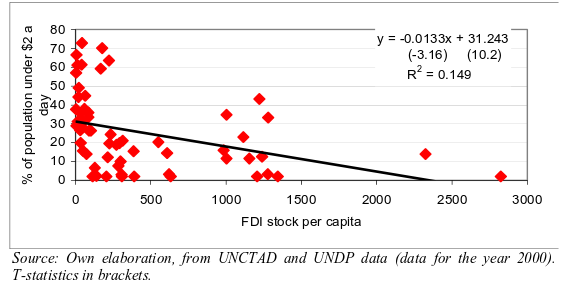
\includegraphics[width=\textwidth, height=\textheight,keepaspectratio]{../figure/fdi_poverty}
\caption{Relationship between FDI and poverty}
\label{fig:fdipoverty}
\end{figure}

Despite the resounding conclusion that the effect of FDI is highly conditional and that investment incentives do not work, why do countries still fixate so much on bringing in FDI instead of developing local absorptive capacity \citep{Blomstrom2002}? For example, Ireland provided foreign investors with lower tax rate, lower land price, and cash grants for R\&D that do not need to be repaid. China also used a tax holiday (two years of no tax and three year of half the normal tax rate) in special economic zones to attract more foreign firms \citep{Telford2001}. We see the same widespread use of investment incentives in Southeast Asia \citep{Fletcher2002}. In Vietnam, the race to offer incentives to foreign firms rages on even among sub-national units, as provincial governments defied the central government's directive and offered extra-legal incentives to FDI firms \citep{Vu2007}. Not only do these measures not work in attracting more FDI, they also deprive countries of revenues that could be spent on improving the local labor quality and investment climate, which are much more conducive to spillover effect and growth.

Thus, my dissertation project focuses on this empirical puzzle: if the positive effect of FDI is uncertain, why is there so much focus on attracting it? If developing absorptive capacity is so crucial to making FDI growth-enhancing, why is it often neglected? To understand this puzzle, I propose that we need to take into account the calculus of the individual bureaucrats and government officials, who may be more interested in the potential rents from foreign firms than the spillover and growth-enhancing effect of FDI. This is a potential reason why we often see countries (i.e. government officials) being so enthusiastic about attracting FDI, yet not so passionate about developing the local capacity that enables FDI to actually have a positive effect on growth.

\begin{figure}[!ht]
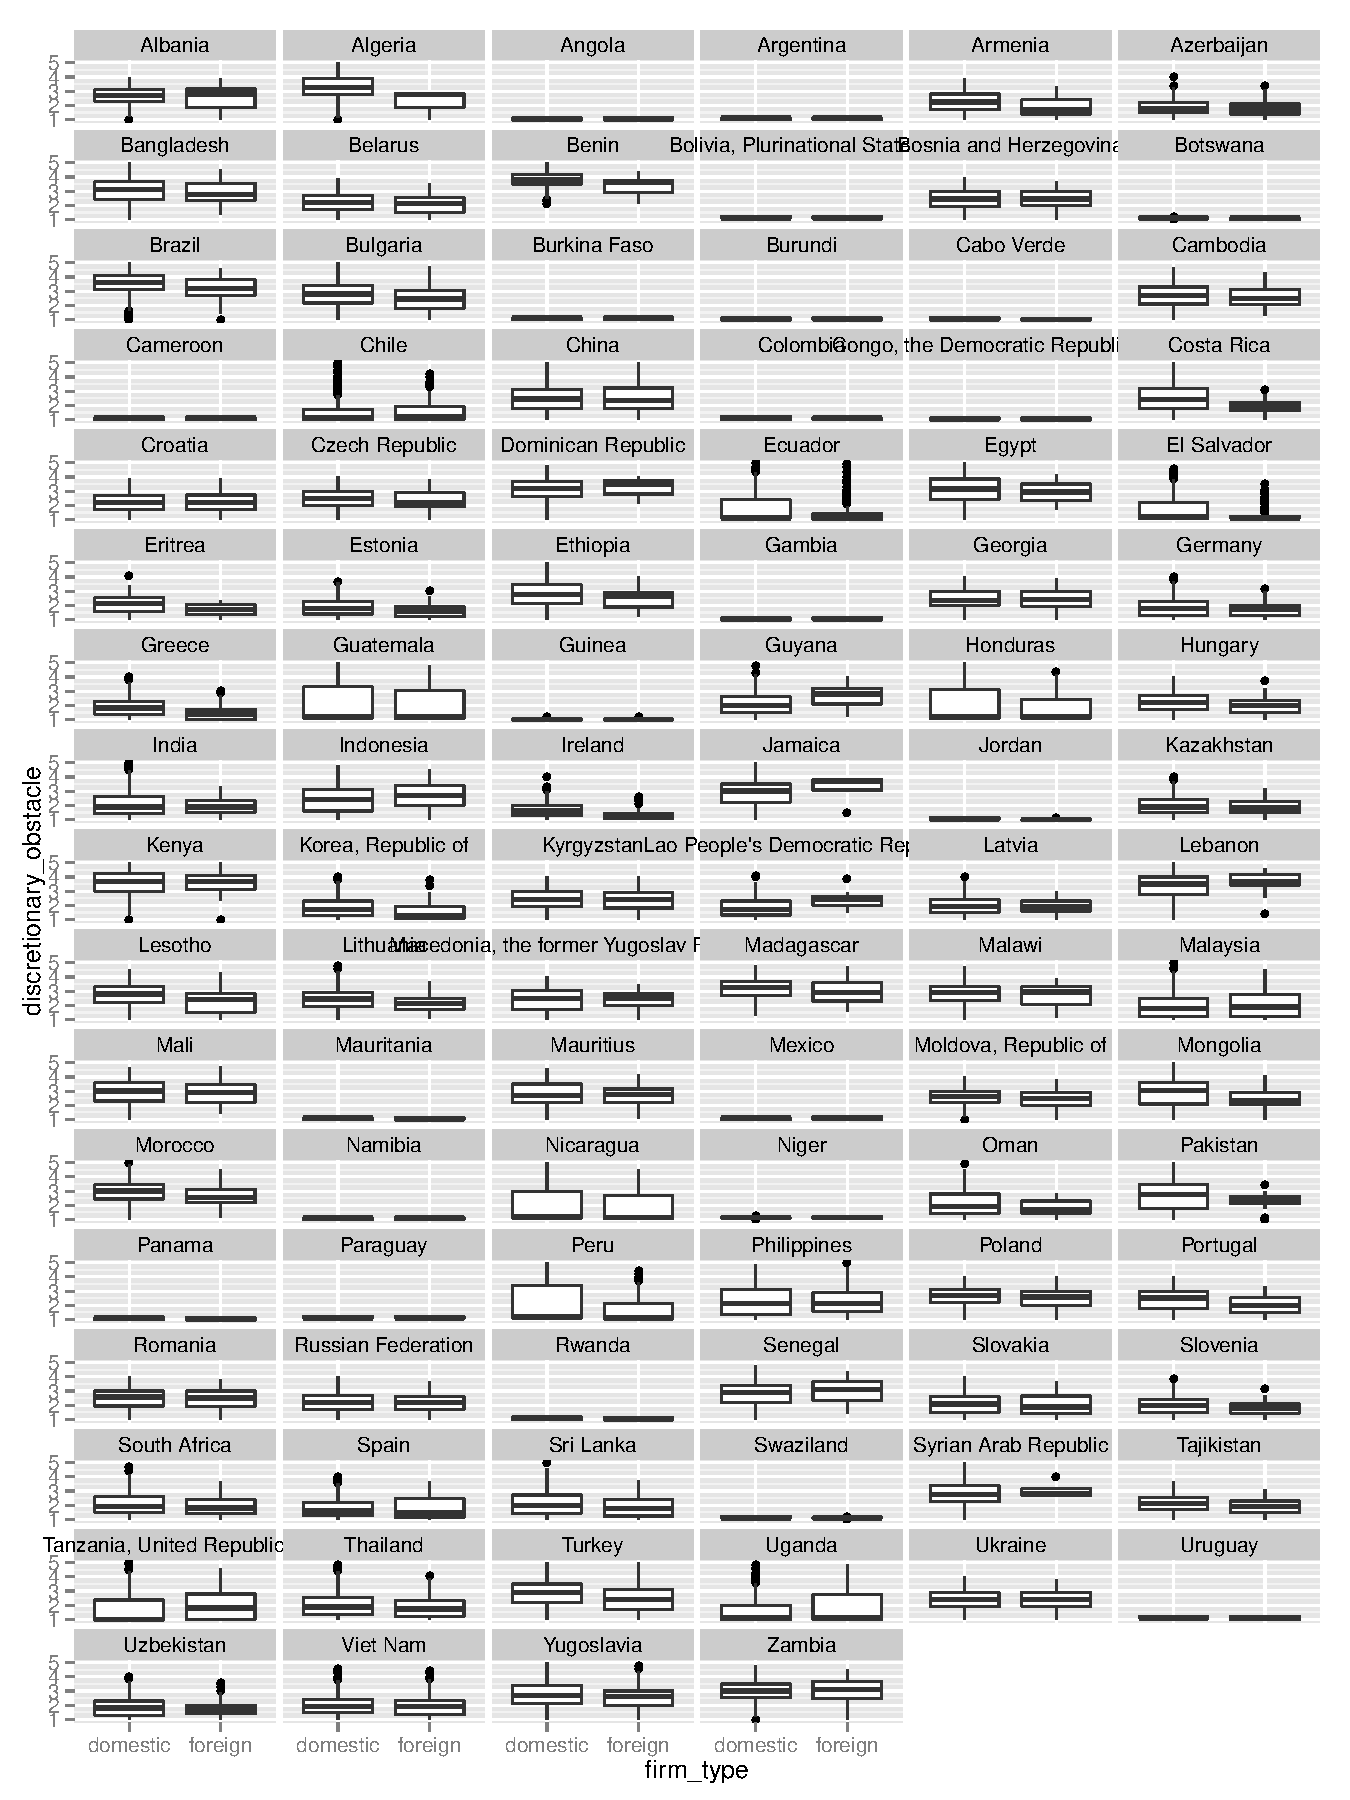
\includegraphics[width=\textwidth, height=\textheight,keepaspectratio]{../figure/fdi_domestic_treatment}
\caption{The treatment of FDI and domestic firms across countries}
\label{fig:fdi_domestic_treatment}
\end{figure}

Starting with this empirical puzzle, my project also sheds light on various related issues. First, it investigates the collusion of FDI firms and host countries' officials, a understudied phenomenon as the existing literature often assumes a foreign firm trying to fend off extortion and harassment from host countries. Second, it examines the political drivers behind private sector development, an issue whose welfare impact is well-known yet whose political determinants are ill-understood. Third, my project looks at the treatment of foreign firms versus domestic firms from a fresh angle. The majority of political science literature has considered FDI the underdog, unfamiliar with the location, susceptible to expropriation, and threatened by the lobbying effort of domestic firms. However, when FDI firms are big and resourceful, they can be an equal partner in the collusive relationship with corrupt officials to the detriment of the domestic sector.


\section{Stylized Facts}
In this section, I present some evidences that motivate the puzzle.

\begin{itemize}
	\item The spillover effect of FDI on growth is highly variable. For example, FDI is found to be growth-enhancing in East Asia, but not in Latin America \citep{Zhang2001}. Similarly, the effect of FDI on domestic investment also varies across countries and regions. FDI is found to crowd in investment in some countries (e.g. Ghana, Senegal, South Korea, Pakistan, Thailand, etc.) but crowd out in others \citep{Agosin2005}.
	
	\item Despite the prevalent concern with discrimination against foreign firms, the Wold Bank Enterprise Survey finds that foreign firms actually face fewer obstacles while doing business \citep{Batra2003}. The gap in the treatment of foreign and domestic firms also varies across countries (\Cref{fig:fdi_domestic_treatment}).
	
	\item The correlation between corruption and FDI is negative. However, there is a lot of unexplained variance at the high end of FDI. Countries with low level of FDI are always very corrupt, but countries with high level of FDI can be as well (\Cref{fig:fdi_corruption}).
	
	\begin{figure}[!ht]
	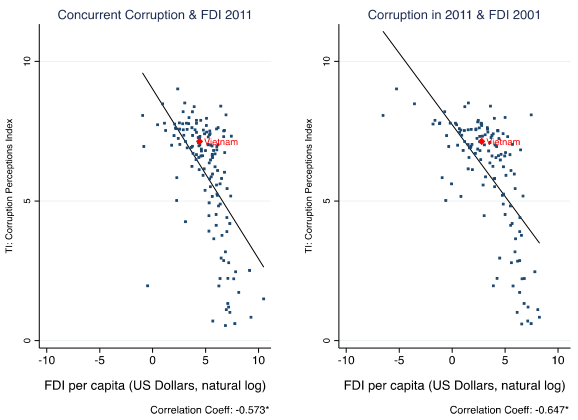
\includegraphics[width=\textwidth, height=\textheight,keepaspectratio]{../figure/fdi_corruption}
	\caption{Source: \citep{Malesky2015}}
	\label{fig:fdi_corruption}
	\end{figure}
\end{itemize}

A closer look into the level of corruption across industries also suggests a negative relationship between spillover and bribe. According to the \citet{TransparencyInternational2011}'s Bribe Payer Index, which measures the propensity of firms from industrialized countries bribing abroad, the most corrupt sectors are public works contracts, utilities, real estate, oil and gas, and mining. These sectors are most vulnerable to corruption due to a lack of competition and a high level of government involvement. They also tend to be less conducive to spillover due to the winner-take-all structure of the industry \citep[138]{UNCTAD2001}. For example, in real estate, utilities, or mining, if scarce resources and contracts can only be won by large foreign firms, then these firms will capture the rent and perpetuate their market power while relegating local contractors to low-value added tasks.

In contrast, the least corrupt sectors are agriculture, light manufacturing, civilian aerospace, IT, and banking and finance. Among these, some are high tech industries (e.g. aerospace, IT) that governments may prioritize to facilitate spillover. Others have low barriers to entry and a divisible production process, both of which are conducive to domestic sourcing (e.g. agriculture, light manufacturing) \citep{TransparencyInternational2011}.

Beyond these broad strokes, the relationship between spillover and corruption emerges in more granularity within the same sector and across countries. For example, despite the stereotype as a high corruption, low spillover sector, the mining industries in Chile, Ghana, and Mozambique have substantial variation of spillover according to the host country's level of corruption. According to the \citet{TransparencyInternational2014}'s Corruption Perception Index, Chile, Ghana, and Mozambique rank 21, 61, and 119 out of 175 countries on control of corruption. Correspondingly, according to surveys of mining firms, Chilean foreign mines ``have the greatest proportion of domestic suppliers and carry out more valued-added activities in-country than [foreign mines] in Ghana and particularly more than in Mozambique'' \citep[127]{Farole2014}. The high level of FDI spillover in Chilean mining may be due to its developed economy and competent base of local suppliers. However, this does not explain the difference between Mozambique and Ghana, two countries with a similar level of GDP per capita.

Importantly, Ghana and Mozambique differ not only in the level of spillover, which can be influenced by economic forces outside the government's strategic decision. In addition, the two governments also diverge in their policies to promote supply chain linkages between foreign and domestic firms. In Ghana, the government worked with the private sector to develop regulations that put real teeth into the local content requirements in the Ghana Minerals and Mining Act (2006). According to these regulations, foreign mining firms are required to develop a five-year local procurement plan, including targets and strategies to develop domestic supplier capacity. These is also clear evidence that the government enforces these rules by striking at the profitability of the firms: when bids are within two percent of prices, the bid with the highest local content shall be selected. In stark contrast, Mozambique shows no commitment to local supplier development either in its Mining Law (2002) or Mining Regulations (Decree no.62/2006) \citep[137]{Farole2014}.

This example shows that if a government wants to induce spillover from foreign firms, it can. Even though policies that affect the profitability of the foreign firms, such as local content requirement, are technically not allowed under the national treatment principle of the WTO, there are many loopholes and little enforcement \citep{Hufbauer2013}. Indeed, Ghana itself has been a WTO member since 1995 and a GATT member since 1962. Therefore, the interesting question is not whether the government can extract spillover from FDI, but under what conditions would it want to do so.


\section{Theory}
\subsection{Actor and choices}

The model has one strategic actor: a government official. This official has control over a certain endowment (e.g. market access, cheap labor) that is attractive to foreign firms.\footnote{I define  \textit{foreign firms} as firms with over 50\% ownership belonging to private foreign individuals, companies, or organizations} Foreign firms that invest in the official's territory turn this endowment into profit via their productive activities. Firms then share the value added with the official in exchange for access to the endowment. 

Firms share the benefit with the official in the form of a two-good bundle: 1) technological spillover and, 2) private benefit (to the official). \textit{Technological spillover} is the beneficial effects of foreign firms' technological knowledge on the productivity and innovative ability of private firms. The official cares about the technological spillover of FDI because it is a crucial ingredient in improving total factor productivity and generating long-term growth, which in turn, brings electoral or career benefits. \textit{Private benefit} that firms offer to the official can come in many forms, both illegal (e.g. bribe, kickback) and legal (e.g. campaign finance contribution, informal network with foreign firms that leads to contracts for friends and families).

The essence of the dissertation project is to determinte how the official chooses the mix of these two goods, i.e. technological spillover and private benefit.

\subsection{Government official faces a budget constraint}

There are two reasons why there exists a budget constraint that prevents the official from getting as much spillover and private benefit as he wants.

First, since the endowment that the official commands is finite, it imposes a constraint on the amount of FDI that the official can attract.

Second, given a fixed amount of FDI, there is a trade-off between spillover and private benefit. In other words, if the official wants more of one good, he has to give up some of the other. To induce spillover, governments frequently impose on foreign firms conditions such as forming a joint venture or local content requirement. These conditions constrain firms' options and their ability to optimally use their physical and management capital, reducing their revenue and profitability. Similarly, when firms are forced to offer private benefit to officials (e.g. bribes, contracts with officials' relatives), they suffer from both an upfront cost as well as the cost of uncertainty (as these private benefits are frequently informal, not transparently encoded, and thus abstruse to foreign firms). For this reason, offering officials private benefit increases firms' expenses and thus also reduces profitability. Given that firms are constrained to maintain a minimum amount of profit (akin to reservation wage) that justifies investing in the country, if a firm offers more private benefit to the official it will have to bring less technological spillover, and vice versa.

One may argue that there are foreign firms that voluntarily produce spillover and this is not mutually exclusive from offering private benefit to the officials. However, such cases are rare because high-tech firms want to keep their technology proprietary. Due to scale and sophistication, foreign firms would also source from established international suppliers and only rely on local suppliers for standard commodity goods at arms-length, which doesn't generate as much spillover as personal contact (e.g. training, quality assurance assistance, financing assistance). FDI firms voluntarily source from local suppliers only when the availability and quality of local suppliers are not far from international quality, and in these cases there's less need and room for spillover. Another scenario that leads to foreign firms voluntarily producing spillover is when they specifically target the local market: in this case, the qualilty requirement is not too stringent, the quantity not too large, and there is a need for rapid local customization. However, in this case, market oriented FDI firms can displace local firms, and the benefit of spillover is offset and can lead to negative spillover \citep{Mody2004}.

Combining the two facts that, 1) the size of the bundle is limited by the official's endowment, and 2) the official has to give up one good to get more of the other from firms, a budget constraint exists over this two-good bundle.

While FDI does bring other benefits, e.g. jobs and capital, the theory intentionally focuses on technological spillover and private benefit for both substantive and theoretical reasons. Substantively, technological spillover increases total factor productivity, which is key to sustaining long-term economic growth when capital has diminishing return. While the literature has mainly focused on the quantity of FDI attracted, development agencies and governments have paid much attention to the issue of technological spillover. 

Furthermore, the implication of a spillover-vs-private-benefit trade-off is very different from that of a spillover-vs-capital/job trade-off. In the later case, one can count on the official to shift towards attracting FDI with high technological spillover as his country gradually grows and is in less immediate need of capital and job creation. The growth trajectory of a country is guaranteed to be positive in this scenario, fueled by FDI's capital injection in the earlier stage and sustained by FDI's technological transfer in the later stage. However, if the trade-off that the official considers is between spillover and private benefit as my project theorizes, then one cannot count on the official to take such benevolent action.

Theoretically, since technological spillover is key to growth, my theory about the official choosing the spillover-vs-private-benefit bundle speaks to the age-old research question: ``Why are some governments corrupt, some growth-promoting, and yet others are both?'' While such question is massive both in its importance and its difficulties, my project approach FDI's spillover effect as a mid-size problem with several mid-level theories, where the model of an official considering the mix of benefits brought by a FDI project is not too abstract from the real-world investment process to be fictional. With the theory well delineated within the topic of FDI, we can pinpoint the parameters that affect the budget constraint and the official's preference over spillover and private benefit as follows.

\subsection{Parameter 1: Official's endowment determines the size of the budget constraint}

Since the official uses his endowment to attract FDI, with more endowment the official will be able to get both more technological spillover and more private benefits. In other words, his budget constraint will shift to the right (\Cref{fig:budget_constraint}). This feature of the model captures the fact that officials in a country with a lot of endowment have a much better bargaining leverage vis-a-vis the foreign firms and can extract both spillover and private benefit (e.g. China).

\begin{figure}[!ht]
	\centering
    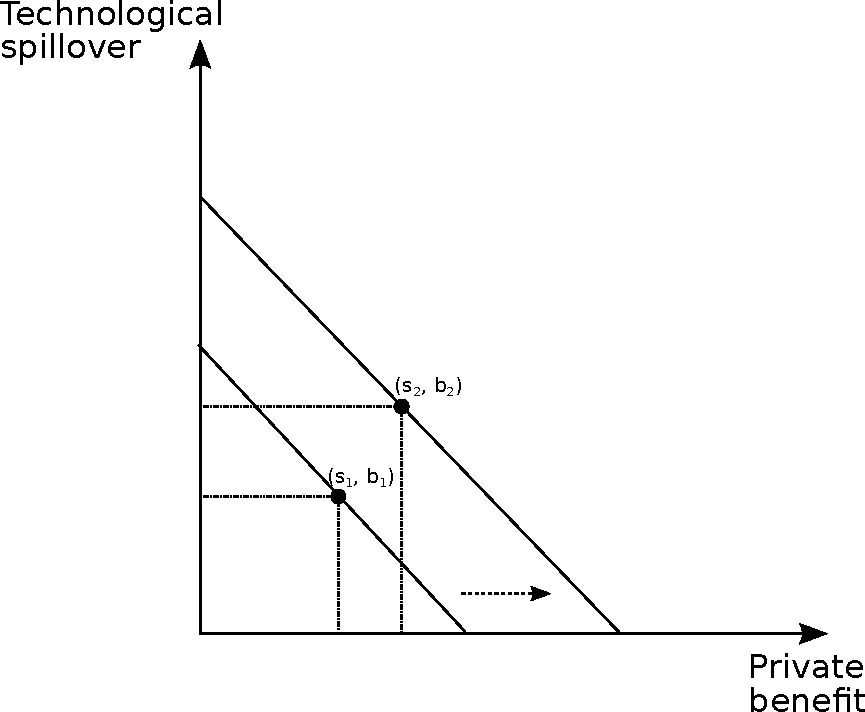
\includegraphics[width=0.75\textwidth, height=0.75\textheight,keepaspectratio]{../figure/budget_constraint}
    \caption{When an official has more endowment, his budget constraint shifts from left to right. He is now able to afford the $(s_2, b_2)$ bundle, with $s_2 > s_1$ and $b_2 > b_1$.}
    \label{fig:budget_constraint}
\end{figure}

\subsection{Parameter 2: price of spillover and private benefit determines the intercept and the slope of the budget constraint}

Given a fixed amount of endowment, the two intercepts of the budget constraint are determined by the ``price'' of the two goods, i.e. how easily the official can obtain technological spillover and private benefit from the foreign investors. If a good becomes harder to extract from foreign firms, the official can afford less of it and the corresponding intercept shifts inward (\Cref{fig:relative_price}). Alternatively, we can think of the slope of the budget constraint as the relative price of the two goods.

Substantively, the ``price'' of technological spillover depends on both the nature of the sector as well as the absorptive capacity of the local economy, which I define as the presence of private firms that are able to absorb technology from foreign firms.\footnote{I define \textit{private firms} as firms with over 50\% ownership belonging to private domestic individuals, companies, or organizations} Consider two channels through which technological spillover happens. First, private firms enter into the supply chain of foreign firms, improving their productivity by imitating the higher production standards or management techniques of foreign firms. For this to happen, it is necessary to have a wealth of private firms that are technologically capable to enter the supply chain. The feasibility of such outsourcing is also sector-specific, e.g. whether the production process is divisible into units, or whether the technology has matured enough for subcontracting. Second, local employees employed by foreign firms may learn from their experience and transfer that knowledge when they move to private firms. For this to happen, private firms must also be technically advanced enough to make use of and compete for this high quality labor from the foreign sector.

The ``price'' of private benefit substantively means how easily the government officials can extract these benefits from the foreign firms. One example of such parameter is the origin of the foreign firm. Firms that come from countries where corruption is more common or accepted would be more adept at providing private benefit to official and more willing to do. In contrast, firms from countries that have signed onto the OECD anti-bribery convention would be more hesitant to bribe given the punishment that they may face from their home governments.

Changing prices of the two goods will shift the budget constraint and, holding the indifference curve constant, have implications for the mix of two goods that the official chooses.

\begin{figure}[!ht]
	\centering
    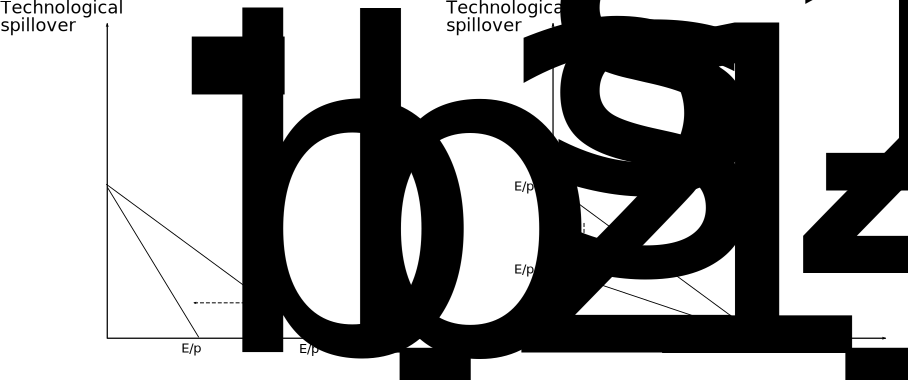
\includegraphics[width=\textwidth, height=\textheight,keepaspectratio]{../figure/absorptive_capacity}
    \caption{In the left panel, the intercept for private benefit moves from the right to the left as its price increases. In other words, $\frac{E}{p_{b2}} < \frac{E}{p_{b1}}$ because $p_{b2} > p_{b1}$. Similarly, in the right panel, as it becomes more difficult to extract spillover from foreign firms, the intercept moves down.}
    \label{fig:relative_price}
\end{figure}

\subsection{Parameter 3: The official's time horizon determines the shape of his indifference curve}

The official has a convex indifference curve, meaning that there is decreasing marginal utility to both spillover and private benefit. This assumption is standard and makes intuitive sense. As the official accumulates more private benefit, there are fewer things worth spending on as his consumption is satiated and produces less utility. Similarly, when more technological spillover happens, it becomes less of a bottleneck to the economy. Thus, voters (or the official's higher-ups) become less concerned with the issue and it brings less electoral (or career) benefits.

The shape of the indifference curve denotes the relative weight the official assigns to the two goods, spillover and private benefit. When the curve is steep, it means that the official is willing to trade a lot of spillover for a small increase in private benefit. Vice versa, a flatter curve indicates that the official values spillover more (\Cref{fig:indifference_curve}).

Politically, the steepness of the indifference curve depends on the time horizon of the official. This is because technological spillover takes time to happen and increase economic growth whereas private benefit is immediate. The longer the time horizon, the more heavily does he weigh technological spillover effect. For example, in \Cref{fig:indifference_curve}, the blue indifference curve is flatter and signifies more weight assigned to spillover. In that case, the official chooses a bundle that has more spillover and less private benefit (i.e. $s_1 > s_2$ and $b_1 < b_2$). Political factors that influence the official's time horizon may include term limit, the stability of the regime, or the probability of electoral success. 

\begin{figure}[!ht]
	\centering
    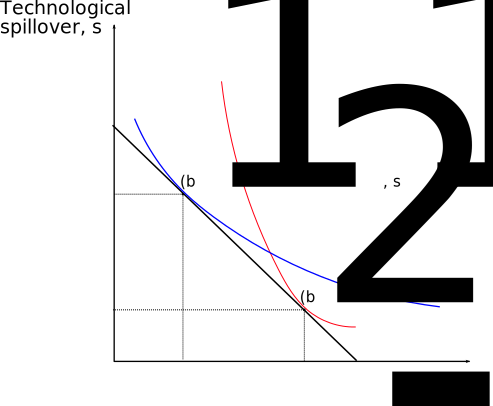
\includegraphics[width=0.75\textwidth, height=0.75\textheight,keepaspectratio]{../figure/indifference_curve}
    \caption{The blue indifference curve shows that the longer the official's time horizon, the flatter his indifference curve, and he will choose more spillover and less private benefit.}
    \label{fig:indifference_curve}
\end{figure}

\subsection{Literature on corruption and FDI}

Regarding private benefit for the officials, I focus on corruption, i.e. bribe and informal fees, given the ubiquity of the practice in developing markets and wealth of data collected on this issue from cross-national business surveys. 

The majority of literature on the relationship between corruption and FDI focuses on showing that a high level of corruption deters FDI \citep{Wei2000, Hakkala2008, Al-Sadig2009}. A smaller literature examines the behaviors of foreign firms that choose to invest in a highly corrupt environment. It argues that foreign firms can help reduce corruption in host country via regulatory pressure effect, demonstration effect, and professionalization effect \citep{Kwok2006}; or via competing away the rents of the domestic firms, reducing the supply of bribes \citep{Sandholtz2003}. In these works, corruption between the host government and the foreign firm has been conceptualized as \textit{predatory}.

My research offers a new perspective, recognizing that, compared to domestic firms, foreign firms always have the freedom to move out of the country or at least stop bringing in capital. Therefore, the exchange between the government and foreign firms are always more voluntary compared to private firms. In this angle, corruption between the government and the foreign firm can be \textit{collusive}, with government officials getting bribe and foreign firms getting exclusive access to resources controlled by the officials (e.g. an expedited bureaucracy or privileged use of public resources) \citep{Hellman2002}. Indeed, there are evidence of foreign firms bribing to get an upper hand in the local market \citep{Barstow2012} or to pursue rent in protected industries \citep{Malesky2015}. 

Such collusive corruption between the government and foreign firm can be the key to explain the puzzle why governments may want to attract a lot of FDI despite the lack of developmental impact. (Corrupt) institutions matter, but not only to \textit{how much} FDI a country can attract as the literature has studied, but also \textit{which kind}.


\subsection{Empirical implications and identification strategy}

In the sections that follow, I contextualize the general theory presented above, building three mid-level theories that map each of the three parameters to a specific empirical context. I also briefly discuss the identification strategy, leaving more operationalization and data availability details for the later Research Design section.

The three parameters in the model and their empirical implications are:

\begin{itemize}
\item \textit{``price'' of spillover}: sectoral and industry variation in the level of potential spillover affects the official's choice of the spillover-bribe bundle.

\item \textit{``price'' of private benefit}: Phase 3 enforcement of OECD's anti-bribery convention makes firms from member countries more hesitant to bribe, raising the cost of bribery and resulting in less bribe and more spillover.

\item \textit{time horizon}: term limit reduces the time horizon of Vietnamese provincial officials that are close to retirement, leading to less spillover and more bribery.
\end{itemize}

\section{Research Design}
\subsection{Measuring the main dependent variable: spillover effect}
\label{sec:measure_spillover}

\subsubsection*{Measuring spillover indirectly}

Similar to how growth economists start endogenizing technological change, FDI researchers investigate how technology spillover from FDI may happen instead of assuming its inevitability \citep{Romer1994}. Several channels for spillovers have been proposed, some of which suggest an indirect measure of technology spillover.

These channels are:
\begin{itemize}
	\item imitation:  private firms may reverse engineer a production or management technique \citep{Wang1992}, which is facilitated by backward linkage between local and foreign firms \citep{Javorcik2004}. This motivates my first measure of spillover effect: \% of private firms that participate in contracts with foreign firms.
	\item competition: similar to the effect of competition from arm's length trade on productivity, the presence of foreign firms in the domestic market put pressure on local firms to reduce inefficiency \citep{Glass2002}.
	\item export demonstration: foreign firms are more knowledgeable about exporting, which involves high fixed cost to set up a distribution and transport infrastructure, or learning about foreign taste and regulatory environment. Domestic firms can learn this ``export know-how'' from foreign firms \citep{Aitken1997}. This motivates my third measure of spillover effect: \% of private firms that export.
	\item skills acquisition: workers trained in foreign firms bring along their human capital when they move to domestic firms \citep{Djankov2000}. This presumes a healthy domestic sector that can offer competitive wages to workers.
\end{itemize}

Among these channels, \textit{imitation} and \textit{export demonstration} forms the theoretical basis of my two proxy measurements of spillover:
\begin{enumerate}
\item frequent business contacts between foreign and domestic firms,
\item percentage of domestic firms engaging in export
\end{enumerate}

\subsubsection*{Measuring spillover directly}

As standard in the economic literature that studies whether there is a spillover effect for FDI, we can also measure spillover directly. This is done in two steps \citep{VanBeveren2012}.

\begin{itemize}
\item First, measure the level of technology or productivity of a firm.

Level of technology: R\&D spending

Level of productivity: Consider the familiar Cobb-Douglas production function:

\begin{align}
Y &= AL^{\alpha}K^{\beta}
\end{align}

where $Y$ is value added, $A$ is total-factor productivity (TFP), $L$ is labor, and $K$ is capital. $y$, $L$, and $K$ are observable, while $A$ is not. Log transform both sides of the equation, we attain a linear form:

\begin{align} \label{eq:cobb_douglas_linear}
y &= a + \alpha l + \beta k
\end{align}

where the lowercase variables are the log-form of the uppercase variables (e.g. $y = \log(Y)$ and so on). \autoref{eq:cobb_douglas_linear} can then be estimated with OLS:

\begin{align} \label{eq:cobb_douglas_OLS}
y_i = \beta_0 + \beta_1 l_i + \beta_2 k_i + \epsilon_i
\end{align} 

where $\beta_0$ is the average total-factor productivity of all firms and $\epsilon$ is the firm-specific deviation from that mean. From the estimated coefficients of \autoref{eq:cobb_douglas_OLS}, we can estimate firm-level TFP as follows:

\begin{align}
a_i &= \hat\beta_0 + \hat\epsilon_i \\
A &= \exp^{\hat\beta_0 + \hat\epsilon_i}
\end{align}

\item Having estimated firm-level TFP (or technology), we then regress TFP (or technology) on the presence of FDI in a country / sector. FDI presence can be measured as:
\begin{itemize}
\item amount of FDI or number of foreign firms in a country (sector). This measure focuses on the horizontal, or intra-sector, linkage of FDI
\item number of foreign firms that the domestic firms are in contact with. This measure focuses on the vertical, or inter-sector, linkage of FDI
\end{itemize}
\end{itemize}


\subsection{``Price'' of spillover: sectoral and industry variation in potential for spillover}

As implied in the theory section, when the ``price'' of spillover is high (i.e. it is difficult to obtain spillover due to the country's absorptive capacity or sector-specific characteristics), the government official would choose a bundle that has more private benefit than spillover (\Cref{fig:price_of_spillover}). 

\begin{figure}[!ht]
	\centering
    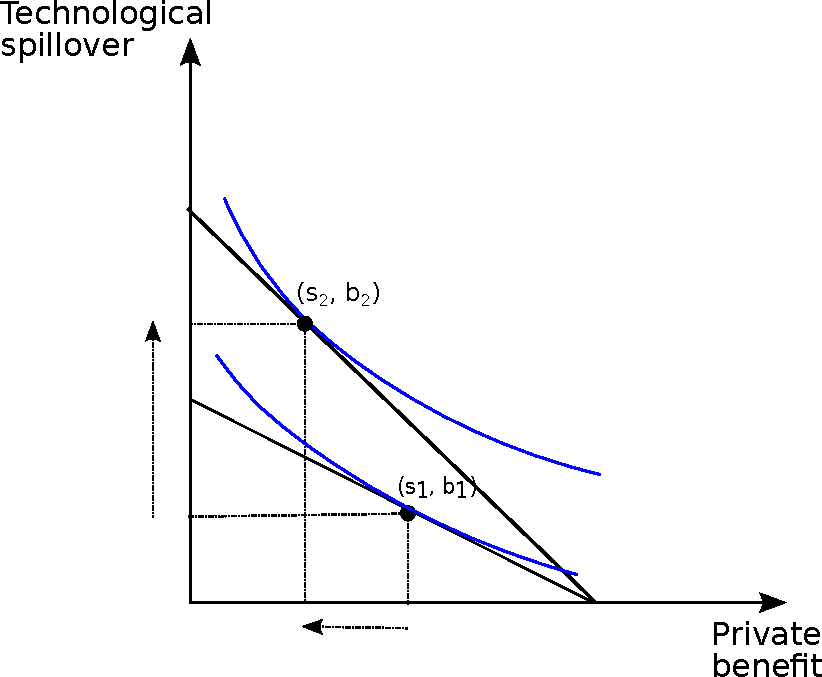
\includegraphics[width=0.75\textwidth, height=0.75\textheight,keepaspectratio]{../figure/price_of_spillover}
    \caption{As the ``price'' of spillover decreases, the official can get a larger amount of spillover given the same budget (i.e. the y-intercept of the budget constraint shifts up) Comparing the bundle $(s_1, b_1)$ and $(s_2, b_2)$, we see that the new bundle has more spillover and less bribe.}
    \label{fig:price_of_spillover}
\end{figure}

Here I focus on industry-specific characteristics that either facilitate or hinder spillover.\footnote{Absorptive capacity, or the ability of private firms to learn from their interaction with foreign firms, is also a very important factor in determining spillover. However, given the time-varying nature of absorptive capacity, not to mention the fact that official and firms can strategically invest to improve absorptive capacity, it is much harder to have a research design studying absorptive capacity that can claim exogeneity.} Due to the divisibility of its production process, manufacturing firms tend to engage more local suppliers and generate more spillover effect than primary and tertiary sectors. In addition, within each sector there is a wide variation across industries to be exploited as well. For example, in manufacturing, food processing can have a high amount of spillover due to the sourcing of raw materials and packaging, whereas in textile and automotive industries (which require high level of technological sophistication), it is harder for foreign firms to work with local suppliers. Similarly, in tertiary sectors, finance, trading, tourisms and utilities are is generally not divisible into discrete stages to subcontract. Yet service industries such as retailing and construction have more opportunities for input suppliers \citep[138]{UNCTAD2001}.

This leads us to the following hypothesis:

\begin{quote}
Hypothesis: Government official will pursue less bribe from firms in industries where it is easier to generate spillover
\end{quote}

While such variation across industries is clear conceptually, measurement is thorny given the many factors that can affect the potential for spillover. In addition, there is an endogeneity problem as the potential for spillover may itself be affected by the level of corruption in that industry. For example, an industry plagued by collusive relationship between the official and foreign firms does not offer an enabling environment that allows private firms to develop their absorptive capacity. The endogeneity problem is compounded if the official strategically decides whether to invest and improve absorptive capacity, in which case it is not even clear which direction is our estimate biased.

To address both of these measurement and endogeneity issues, I will use the variation in technological spillover across industries in the United States as the instrumental variable.\footnote{The United States is considered due to its high quality economic data. Alternatively, for each country, I can use a comparable country in the same region or the same developmental stage to formulate the instrument} The assumption is that the level of technological spillover in a US industry only correlates with the level of bribe in another country's industry through the latent factor that is the industry-specific potential for spillover.

To measure corruption, presence of FDI, and treatment of firms across countries, I utilize the World Bank's Enterprise Survey (ES), which includes a wealth of firm-level data across 125 countries, spanning various topics from investment, labor, to business-government relation \citep{WorldBank2015}. The Enterprise Survey uses stratified random sampling (using three strata: firm size, business sector, and region) in order to ensure representativeness. The survey data comes from face-to-face interviews with upper management and is anonymized to ensure confidentiality at all times.\footnote{For more on the methodology of the Enterprise Survey, visit \url{http://www.enterprisesurveys.org/methodology}} This dataset has a wealth of firm-level data that helps us operationalize key concepts as detailed below.

Operationalization of variables:
\begin{itemize}
\item FDI spillover: See \Cref{sec:measure_spillover}. The level of FDI by sectors is available via the Enterprises Survey dataset.\footnote{It would be better if there is UNCTAD data for FDI by sector, since the Enterprize Survey is not designed to account for all FDI inflow. Without weights, it is difficult to accurately get the population of foreign firms from the ES' sample of foreign firms.}

\item Corruption: can be measured in two ways. 1) Firms' perception about corruption as an obstacle. This measure is frequently used but is not accurate since firms' perception of corruption depends not only on the level of corruption but also the characteristics of firms. 2) Hard measure of prevalence and depth of bribes, e.g. ``Was an informal payment expected or request (when applying for a license)?'', ``How much do establishments like this one give in informal payments?'' 
\end{itemize}
\subsection{Project 2: ``Price'' of private benefit---cost of bribing for foreign firms}

As discussed in \Cref{sec:theory_budget_constraint_slope_and_intercept}, when the ``price'' of private benefits is high (i.e. it is costly for the firm to offer the official private benefits), the official would choose a bundle that has fewer private benefits.

This theoretical claim generates many substantive predictions that we can test, each involving a factor that affects the cost of bribing for firms. For example, foreign firms that come from a corrupt home country may have more experience with bribing and thus would incur less information cost if they bribe.

Here I focus on the Phase 3 (Enforcement) of the OECD Anti-Bribery Convention (ABC) as an exogenous increase in the cost of bribing for firms from member countries. In December 1997, all members of OECD and an additional five non-members, accounting for nearly 61\% of world trade, signed the ABC. The ABC criminalizes the bribery of foreign public officials and upholds its principles with a peer-monitoring system, in which member countries visit and review one another's legislation and implementation. According to legal experts, these reports are often quite harsh and effective in shaming countries into improving their practices \citep{Tyler2011}.

Important for my research design, in December 2009 the OECD's Working Group on Bribery (WGB) annouced that following Phase 1 and 2 (Evaluation and Assessment) there would be a Phase 3 (Enforcement). The goal of Phase 3 is to continually monitor countries' anti-bribery practices and to exhort inactive enforcers. Noticeably, Phase 3 also removed a previous exception that allowed firms to make ``small facilitation payment'' \citep{Strauss2013}. Researchers have argued that following the announcement of Phase 3, member countries ramped up enforcement to avoid a negative review, and causing their firms to reduce bribery abroad \citep{Malesky2015b}. 

In sum, I hypothesize that

\begin{hyp}
After the Phase 3 (Enforcement) of OECD's Anti-Bribery Convention, firms from member countries have more spillover and fewer bribes than firms from non-member countries.
\end{hyp}

In addition,

\begin{hyp}
After the Phase 3 (Enforcement) of OECD's Anti-Bribery Convention, firms from member countries with stronger enforcement have more spillover and fewer bribes than firms from member countries with weaker enforcement.
\end{hyp}

To test the effect of the ABC, I use data from an annual survey of FDI firms in Vietnam, which is an ideal empirical setting for several reasons. First, Vietnam attracts FDI from a wide range of countries, including both member and non-member countries of the ABC. Second, given that FDI to Vietnam only accounts for a small fraction of ABC countries' total foreign investment, it is plausible that Vietnam is not a major factor driving the initiation of Phase 3. Therefore, the announcement of Phase 3 serves as an exogenous shock to the cost of bribery for firms from ABC member countries. With these firms being reluctant to offer bribes, we expect officials to become uninterested in extracting private benefits from them. Post 2009, they would be attractive only for their developmental impact, and we should observe them having more spillover effect.

With 2009 as an exogenous shock we have a difference-in-difference design. First, we estimate the difference in spillover between ABC and non-ABC firms, pre-2009. We then find the same difference in spillover post-2009. Subtracting these two differences, we can estimate the effect of corruption on the level of spillover.\footnote{An alternative design looks at the difference between ABC and non-ABC firms that \textit{enter} Vietnam pre- and post-2009. This design will have fewer firms in the sample but could be more appropriate if we think that the spillover-bribe bundle is negotiated at the time firms enter Vietnam and is hard to change later, even with the ABC coming into effect. If so, the change in level of spillover and bribe is caused by the change in the official's selection of firms instead of the adjustment in behaviors of existing firms after 2009.} To operationalize the strength of enforcement among member countries, I use \citet{Heimann2013}'s assessment of the OECD ABC progress.


This project also takes advantage of the list experiment by \citet{Malesky2015} to measure the level of bribery. Indeed, asking directly about firms' experience with corruption is unlikely to get an accurate answer due to sensitivity bias \citep{Coutts2011}. Researchers, including the ES team, often address this problem by framing the question about the experience with corruption of ``firms like yours.'' However, with this technique, firms may not read between the lines and actually answer about the experience of others \citep{Ahart2004}. The unmatched count technique circumvents these issues by not forcing firms to incriminate themselves with corruption.
\subsection{Project 3---time horizon of officials}

As discussed in \Cref{sec:theory_indifference_curve}, an official with a longer time horizon would choose a bundle with more spillover, whereas an official with a shorter time horizon would choose a bundle with more private benefits.

To get a handle on the time horizon of the official, we need to know the options provided to the official within the country's political economic system. Such is a difficult question to study with a cross-national design due to endogeneity issues, stemming from unobservable and unmeasurable differences across political systems. Therefore, at this step, I focus on the case of Vietnam, whose large number of provincial units (63) and their variation in FDI flow serve as an excellent testing ground. Again, here I focus on bribe and informal fees as the main form of private benefit for officials. Such constraint is not problematic for the case of Vietnam, where there is no campaign contribution and revolving door jobs are non-existent.

\subsubsection{The effect of time horizon on the choice of Vietnamese provincial officials} 

The relative weight assigned to spillover versus bribe by the Vietnamese provincial officials is determined by the principal-agent relationship between Vietnam's central and the provincial governments. On the one hand, the central government (i.e. the principal) cares more about the spillover effect of FDI and uses promotion to reward local officials that attract high-spillover FDI. On the other hand, local officials (i.e. the agent) have more opportunities to engage in corruption with foreign firms, and should they decide that the private benefit of corruption is greater than that of promotion, they will prioritize foreign firms that bring bribes over those that have high spillover effects.

The reason behind such difference in the preference of central and local governments is the fact that FDI projects are approved and managed at the provincial level. While the central law may be uniform in the book, its implementation varies widely across sub-national units in Vietnam \citep{Meyer2005}.\footnote{Vietnam's sub-national variation in implementation generalizes well to other cases, such as China \citep{Thun2006}} Therefore, provincial governments hold valuable services for sale to foreign firms. In contrast, the central government is not in charge of approving FDI projects (except those few with national importance) and thus less likely to benefit from corruption than provincial leaders.

In addition, the central government is much more concerned with overall economic growth, which is central to the longevity of the regime \citep{Malesky2008}. It wants to attract high spillover FDI and uses promotion to reward local officials that accomplish this goal. On the other hand, each provincial leader is incentivized to free-ride on the developmental effort of other provinces and of the central to keep the entire regime stable. Therefore, local officials value the spillover effect of FDI only insofar as the opportunities for promotion that it brings.

Fortunately for the central government, the principal-agent problem in this context is partially solved because monitoring is not too difficult. Indeed, the central government can observe the economic performance of the provinces and use personnel management to punish and reward provincial officials \citep{Sheng2007, Li2005}.\footnote{\citet{Shih2012} recently argue that economic performance does not matter to cadre promotion. However, they investigate all members of the Chinese Central Committee, including the central party apparatus, the army, and the central economic bureaucracy. These actors are not the important decision-makers in our theory.} Therefore, the principal-agent problem is only severe when provincial officials are not interested in further promotion to the central government, i.e. when the local official's time horizon is short. This suggests that there will be a variation in the level of FDI's spillover effect across provinces according to provincial officials' interest in promotion. In the research design, I use fuzzy regression discontinuity (RD) exploiting the mandated retirement age of Vietnamese officials, arguing that those that are in their last term have shorter time horizon and less interest in promotion.\footnote{The design is \textit{fuzzy} RD because the shortening of time horizon does not happen so abruptly as after a specific date. Instead, it happens in a time window after the official enters their last term before retirement.}

By looking at this variation in the career interest of provincial officials, my theory contributes a fresh angle to the current literature on the relationship between decentralization and corruption. So far, scholars have only postulated a one-way relationship: either decentralization increases bribery \citep{Fan2009} or reduces it \citep{Guerra2009}. In my model, how decentralization affects corruption is conditional on the local officials' interest in the promotions offered by the central government as carrots.


Three key assumptions in the theory above deserve further examination:
\begin{enumerate}
\item Why wouldn't Vietnam's central government worry that technological spillover would lead to a developed private sector, and consequently to social change that ultimately undermines its rule?

First, there is a large scholarship showing that authoritarian regimes are very adept at using institutions to manage regime outsiders in general and business in particular \citep{Gandhi2006, Gandhi2008, Wright2008, Le2015}. Second, if the legitimacy of the regime rests heavily on delivering economic growth, then the short-term risk of an economic downturn creating instability features much more prominently than the long-term concern with social changes. Third, it is possible to foster economic growth while restricting political freedom (e.g. Singapore). Indeed, growth can make a regime, both democratic and authoritarian, more stable, and creates room for political control \citep{Przeworski1997}.

\item Why don't provincial leaders seek rent from the domestic sector? 

First, Vietnam's private sector was very small when FDI was first allowed into Vietnam. The size and the profitability of the average domestic firm is still smaller than those of foreign firms today. Therefore, there are both fewer rents and more coordination problems if provincial officials want to seek rents from domestic firms. Second, ironically, if officials want to grow the private sector for future rent-seeking, they must promote an enabling business environment that are free from rent-seeking. In contrast, engaging in corruption with large and existing FDI firms is much more convenient. Essentially, corrupt provincial officials have shifted the cost of building a thriving domestic sectors to the home countries of FDI firms and now extract rents from the high productivity and high profitability of these firms. 
\end{enumerate}

In sum, I hypothesize that

\begin{hyp}
In provinces whose leaders are in their last term before the mandated retirement age, there are less spillover and more bribes from the foreign firms.
\end{hyp}

In addition to the fuzzy RD design using term limit, this project also attempts to measure the preference of the official directly with a survey conjoint analysis instead of relying on the observed level of bribe and spillover. Indeed, it is difficult to fully examine the official's utility function with only observational data because what he truly wants may not be fulfilled due to external and unobservable factors. Furthermore, what an official wants from a FDI firm is often hard to tease out completely. A big FDI firm is an attractive source of bribe, but it also brings job and technology. Indeed, perhaps this high multicollinearity is precisely why it is so easy for officials to extract bribe from FDI under the guise of promoting economic development.

To truly get at the utility calculation of provincial officials, I plan to conduct a survey experiment using conjoint analysis to ask provincial officials about their preference between two hypothetical FDI firms \citep{Hainmueller2014}. The characteristics of these firms will be randomly varied across several dimensions: size of labor force, capital, technology age, and most importantly, need for land, which proxies for corruption opportunities.

\subsubsection{Why choose land as a proxy for corruption?}

To discern provincial officials' preference for corruption opportunity versus developmental impact, one must vary the hypothetical FDI project along a characteristic that can only be attractive to officials because of its potential for corruption and not any other reasons. In this regard, the amount of land a project requires is the best proxy for corruption. Since land is an increasingly scarce and expensive resource in Vietnam, acquiring land from current tenants and farmers is a difficult, sometimes violent, process. Therefore, there is neither good developmental nor political reason for local officials to prefer a project that needs a large amount of land. 

In contrast, other characteristics of a FDI project can be preferred by officials for many different reasons. For example, a well capitalized project may signify a large pot of money to dip in, but it may also be attractive for the labor productivity enhancing effect of its capital. Similarly, a FDI firm with a large labor force may need to curry favor with officials to suppress their workers, but it may also be appealing for the jobs it creates.  Unlike those factors, land is unambiguously an indication of corruption opportunities. With a high level of \textit{monopoly} and \textit{discretion}, local officials are able to sell land access, something that investors are eager to buy.

1) Monopolistic control over land supply: At the start of Vietnam's liberalization (under Land Law 1993), any exchange of land between land users and investors must go through the local government. Investors had to negotiate with all levels of local governments (i.e. commune, district, and province level people's committees) to acquire land---a complex process that encouraged investors to use informal procedures and fees to expedite. Importantly, the price of land was solely determined by the local government, which was usually 10-30\% of the market price. Therefore, officials were able to extract bribes with both their gate-keeping and price-setting powers over land.

Subsequent land law reforms (2003 and 2013) attempted to bring the land acquisition process closer to a market approach and lessen the monopolistic control of the local government over land. For example, Land Law 2003 specified two methods for investors to acquire lands: voluntary and compulsory. Under compulsory land acquisition (akin to eminent domain), local governments retain the power to acquire land with compensation then allocate to approved investors. Under the newly-introduced voluntary land acquisition, investors negotiate with and buy from land users in a private market transaction. Despite the option of buying lands from private users, in practice most investment projects tellingly opted for compulsory land acquisition by the state. With the local government's coercive power and legal ability to set compensation value on their side, investors find compulsory land acquisition both faster and cheaper, and thus worth paying for.

Similarly, despite many calls for removing the state's control over land, Land Law 2013 disappointed with its insistence on ``people's ownership'' of land instead of adopting a fully private ownership system. Furthermore, the law preserves the state's right to acquire land for the vaguely defined ``socioeconomic development'' and ``national interest,'' which expansively includes the development of industrial zones.

2) Discretionary allocation of land to selected investors: Opportunities for corruption also arise from two discretionary powers of the local governments. First, land acquired by the government is allocated directly to approved investors instead of through public auction, an option allowed by law but rarely practiced by local governments. Second, in many cases, local officials even modify the existing land use plans according to the suggestions of investors, making available land that was previously not zoned for business development. Without any standard guideline for investor approval, this process relies heavily on personal contacts and is prone to bribery and kickback.

An important symptom of this corrupt practice is the lack of transparency in the land allocation process and decision. Key information, such as the criteria of project approval, the shortlist of investors, the profile of the selected projects and investors, and the (dictated) price of land, are kept among selected investors and a few state officials involved. Even a straightforward compliance with transparency regulation, i.e. the public posting of investment site maps, is not fulfilled. In a 2010 study, DEPOCEN researchers could only access the investment site maps in 2 of the 12 visited provinces \citep{Anderson2011}.\footnote{But Land law 2013 does remove the direct allocation of land to approved project, instead try to increase the number of land auctions. Does this have an effect?}

\subsubsection{Conjoint analysis design}
Please read the following description carefully. Then, please indicate which project you prefer to grant investment license (cap giay phep dau tu).

\begin{center}
  \begin{tabular}{ c | c | c }
    \hline
     & Project 1 (Du an 1) & Project 2 (Du an 1) \\ \hline
    Industry &  &  \\ \hline
    Labor force &  &  \\ \hline
    Capital &  &  \\ \hline
    Land &  &  \\ \hline
    Technology age &  &  \\ \hline
    \hline
  \end{tabular}
\end{center}

If you have to choose, which project do you prefer to grant investment license? Project 1 / Project 2

\begin{itemize}
\item Industry: textile, electronics, automobile, consumer product
\item Labor force: 5, 50, 100, 200, 500 employees
\item Capital:
\item Land:
\item Technology age: 
\end{itemize}
\subsection{Two-sided Matching}

\subsubsection{Hypothesis}

\subsubsection{The two-sided logit (TSL) model}

Intuition: If we have the complete data of all offers from all countries to all firms, we would have been able to figure out the preference.

In real data, we may not have this complete data, only data where firms have already chosen a country.

EM algorithm allows us to find the hidden parameters by iteratively run as follows. First, assume some values for the parameters. Then, calculate the likelihood of the label assignment. Then based on the label assignment, calculate new values for the parameters.

We don't know the preference, nor all the offers. So we assume some params values for the preference, fill in the offersn, then calculate the preference again. Rinse and repeat.

\subsubsection{Data}

\section{Time Line}

\clearpage
\bibliographystyle{chicago}
\bibliography{library}
\end{document}
